% !TEX root=/home/tavant/these/manuscript/src/manuscript.tex

\section{Simplified 1D PIC simulations}
  \label{sec-1DPIC}

  We have seen in \cref{sec-insights} that the secondary electron emission is not responsible for the temperature radial profile.
  Hence, we neglect it in this section.
  The simulations are at low pressure, in which case  the electrons are non-local \cite{bernstein1954, godyak1993}.
  In low pressure bounded discharges, it is well-known that the EEDF is not Maxwellian in both capacitively coupled plasmas and inductively coupled plasmas \cite{mouchtouris2016, godyak2002, meige2006a, dominguez-vazquez2018}, in agreement with \cref{fig-EEDF}.

  The impact of non-Maxwellian EEDF on the electron flux to the wall has been studied by Kaganovich et al. \citep{kaganovich2000,kaganovich2007}.
  They showed that the electron kinetics at low pressure can significantly reduce the electron flux to the wall, in agreement with kinetic simulations.
  The main parameter determining the electron flux was found to be the electron scattering frequency.
  However, to our knowledge no fluid model describes the sheath with non-Maxwellian EEDF.

  The evolution of the electron temperature and the non-locality of the electrons in bounded plasmas has been studied in \citet{meige2006a}.
  The authors showed that the high energy tail of the \ac{EEDF} is depleted.
  They observed that the energy at which the depletion starts correspond to the local plasma potential related to the wall.
  Hence, we will use in this chapter similar physical conditions, in order to compare our results to their observations.

  \subsection{Description of the \acs{1D} simulations}

    We use a 1D PIC simulation of an argon plasma confined between two walls separated by a length $L=10$cm.
    The background pressure is varied between 0.05 and 10 mTorr.
    The direction of the simulation is $x$, and $y,z$ are perpendicular to the simulation domain.

    The same particle source model as in \ac{2D}\ac{PIC} of the \ac{HET} is used.
    In order to compensate the particle losses at the wall, we inject with a spatially uniform probability an electron-ion couple for every ion lost at the wall.
    This corresponds to the following ionization rate:
    \begin{equation}
      S_{iz} = \frac{1}{L} 2 \Gamma_e
    \end{equation}
    with $\Gamma_e$ the electron flux to the wall.
    A second model will be used later, with a self-consistent heating and ionization.

    Monte Carlo collisions (MCC) are still used, but we do not model the particle generation of the ionization process, but only the scattering and momentum transfer.
    As previously, Coulomb collisions are not included in the study as we are at low plasma density (at steady-state the electron density is around $n_e = 10^{15}$m$^{-3}$).

    To satisfy generally accepted accuracy conditions for the cell size and time step \citep{turner2013}, a time step of $3.7\cdot10^{-11}$\,s is used with a cell length of $1.7\cdot10^{-5}$\,m.
    This allows us to resolve properly the plasma frequency $\frac{2 \pi}{\omega_{pe}} = 3.5\cdot10^{-9} $\,s and the Debye length $\lambda_{De} = 3.10^{-4}$\,m.
    Around $300$ particles per cell are used for the simulations, and statistical convergence has been verified for both the cell length and the number of particles per cell.


    \begin{table}
      \centering
      \begin{tabular}{lll}  \toprule
        Parameter & Value & Unit  \\ \midrule
        Pressure $P$ & $0.05,0.1,0.5, 2, 10$ & mTorr\\
        Initial density & $1 .10^{15}$ & m$^{-3}$\\
        $\Te_{, inj}$& 5 & V\\
        Domain length $L$ & 10 & cm\\
        gas & Argon & -\\
        \bottomrule
      \end{tabular}
      \caption{Simulation parameters for the 1D PIC simulations.}
      \label{tab_1DPICParams}
    \end{table}


  \subsection{Simulation results of the \acs{1D} \acs{PIC} simulation} \label{subsec-1DPIC_results}

    \Cref{fig-PIC1} shows the results of the simulation with the parameters of \cref{tab_1DPICParams}.
    We only present in this section the result for neutral pressure $P=0.1$mTorr.
    The results obtained with different pressure show the same characteristics, and the effect of the pressure is further discussed in \cref{subsec-presurseffect}.
    
    \begin{figure}[!htb]
      \centering
      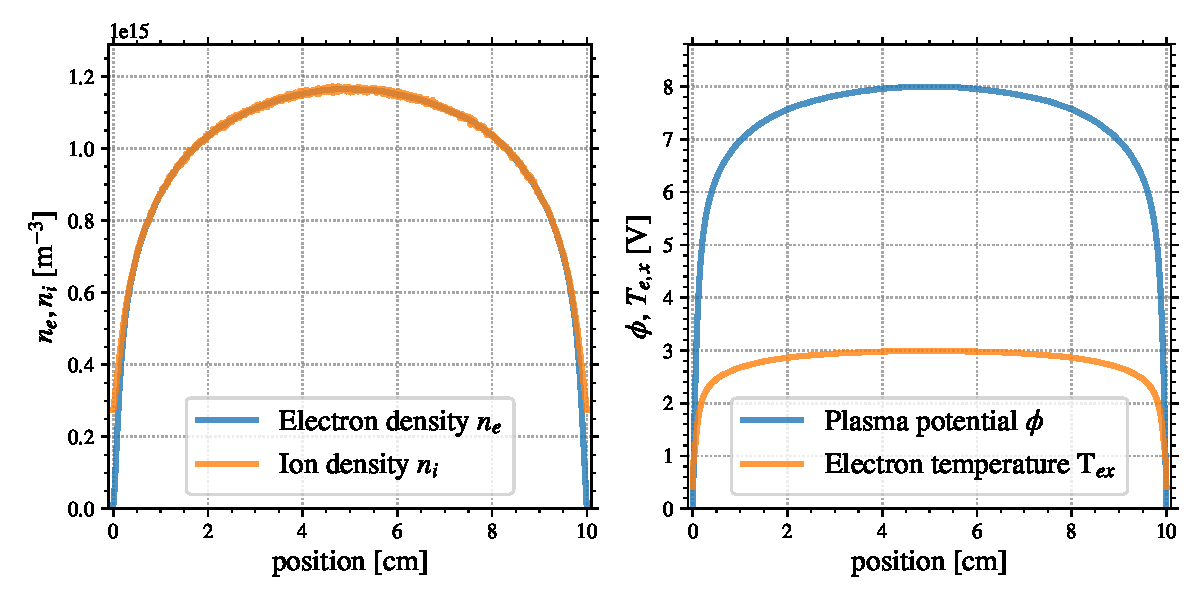
\includegraphics[width=\textwidth]{1D_PIC_summary.pdf}
      \caption{Profile of the electron and ion densities (left) and the plasma potential and electron temperature in the PIC simulation with the parameters of \cref{tab_1DPICParams}, with $P=0.1$mTorr.}
      \label{fig-PIC1}
    \end{figure}


    On the left-hand side we observe the electron and ion density profiles, while on the right the plasma potential and the electron temperature are shown.
    In \cref{fig-PIC1}, the electron and ion densities and the plasma potential feature the usual symmetric profiles with a pre-sheath and a sheath.
    However, while the electron temperature is almost constant in the plasma bulk at the center of the simulation domain, we observe a steep decrease in the sheath.
    The electron temperature gradient should affect the density profile in the sheath and the electron heat flux to the wall.

    \vspace{1em}
    For isotropic distribution functions, it is convenient to introduce the electron energy distribution function (EEDF) $f_{\epsilon}$ \citep{chabert2011}:
    \begin{equation}
    f_{\epsilon}(\epsilon) d\epsilon = 4 \pi v^2 f_e(\vec{v}) dv
    \end{equation}
    It is related to the electron energy probability function (EEPF) $f_{P}$ by
    \begin{equation}
    f_{P}(\epsilon) = \epsilon^{-1/2} f_{\epsilon}
    \end{equation}

    As the distribution function is anisotropic, and since the direction of interest is the $x$ direction, we focus here on $f_{P x}(\epsilon_x)$ the EEPF in the $x$ direction, with $\epsilon_x = \frac{m_e v_{e,x}^2}{2}$.


    \begin{figure}[!htbp]
      \centering
      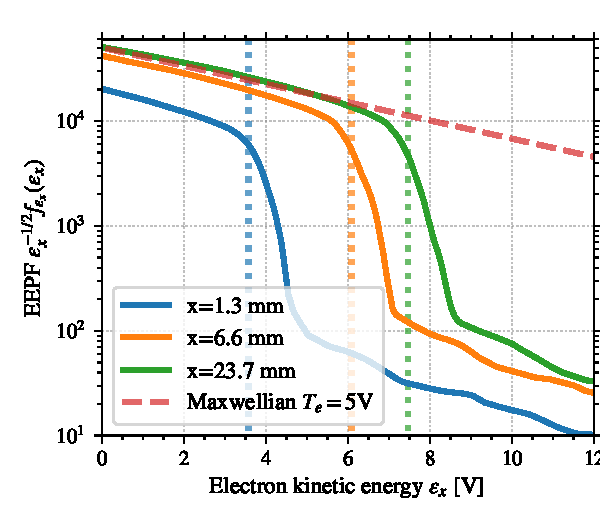
\includegraphics[width=\defaultwidth]{EVDFs.pdf}
      \caption{Electron energy probability function at different positions in the simulation: at $x=1.3,6.6$ and $23.7$ mm in blue, orange and green respectively. Also shown are the Maxwellian distribution of temperature $\Te=5\eV$ (red dashed line), as well as the local plasma potential relative to the wall $\dphi$ (dotted lines). }

      \label{fig-PIC2}
    \end{figure}

    \Cref{fig-PIC2} presents the EEPF measured in the PIC simulations at different positions.
    As the system is symmetric around x=5cm, the positions have been chosen arbitrarily in the left sheath, and their values correspond to the positions of the cell centers.
    We can see that the low energy population ($\ek < e \dphi$) is nearly Maxwellian, of temperature $\Te = 5\eV$ which is the injection temperature $\Te_{, inj}$.
    This population corresponds to the electrons confined by the sheath.
    However, the high energy tail ( $\ek > e\dphi$) is depleted due to the absorption at the wall \citep{meige2006a,kaganovich2007,lafleur2011}.
    This results in a  non-Maxwellian EEPF of temperature, defined with \cref{eq-TeDef}, lower than $\Te_{, inj}$.
    The small population of electrons with very high energy corresponds to the electrons newly generated that have not yet reached the walls.



  \subsection{A model for the EVDF observed}
    \label{sec-twoTe}
    In order to describe the  EEPF seen in \cref{fig-PIC2}, it is possible to use a two-$\Te$ distribution \citep{lafleur2011,mouchtouris2016, zhang2016}:

    \begin{equation}
      f_{Px}(\ek_x) = A \ek_x^{1/2}
    \begin{cases}
      \exp( - \frac{\ek_x}{T_1} -  \frac{\epsilon_b }{T_2}) , \, \ek_x < \epsilon_b \\
      \exp( - \frac{\ek_x}{T_2} - \frac{\epsilon_b }{T_1} ) , \, \ek_x > \epsilon_b
    \end{cases}
    \end{equation}
    with $\epsilon_b$ the energy of the knee, $T_1$ and $T_2$ the two temperatures, and $A$ a normalization constant.
    In the case of absorption by the walls, we can assume that $\epsilon_b = \dphi$ as the absorption only occurs for the electrons of energy higher than $\dphi$.
    For the case of \cref{fig-PIC2}, we find $T_{1}=5$eV and $T_2=0.5$eV.
    This model is closer to the \ac{PIC} EEPF, but neglects the tails of newly generated electrons of high temperature, as we can see if in \Cref{fig-PIC3}.


    \begin{figure}[!hbt]
      \centering
      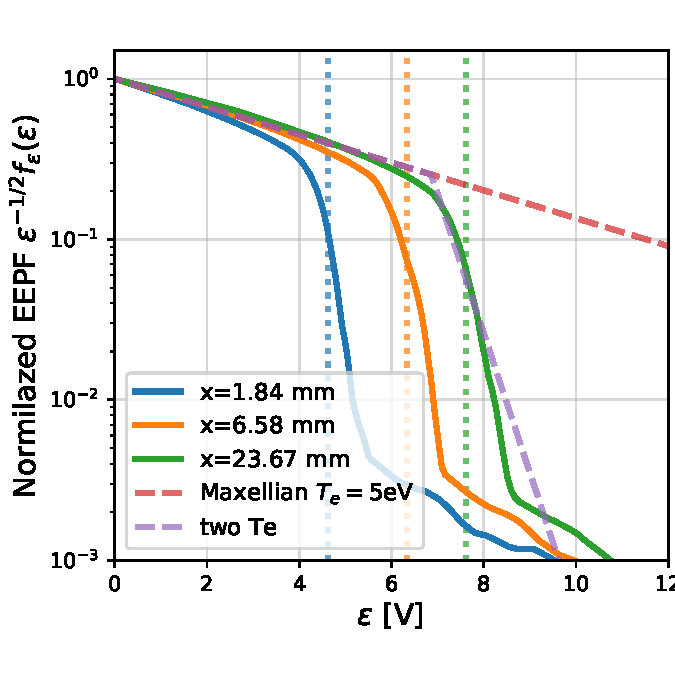
\includegraphics[width=\defaultwidth]{EVDFs_and2Te}
      \caption{Electron energy probability function at different positions in the simulation, as in \cref{fig-PIC2}, but overlaid with a 2-temperature distribution function.}
      \label{fig-PIC3}
    \end{figure}

    In the next section, we investigate a way of taking into account this non-local kinetic phenomenon in a fluid model.
